Chương này trình bày thiết kế và triển khai hệ thống kiểm soát chất lượng không khí trong căn hộ chung cư sử dụng cây trồng trong nhà. Hệ thống được thiết kế theo kiến trúc nhiều lớp gồm lớp cảm biến - chấp hành, lớp truyền thông LoRa, lớp gateway, lớp nền tảng IoT và lớp ứng dụng người dùng. Cách tổ chức này kế thừa hướng tiếp cận của các hệ thống IAQ tích hợp IoT: đo thông số môi trường theo thời gian thực, phân tích dữ liệu trên gateway hoặc cloud, sau đó điều khiển thiết bị nhằm duy trì điều kiện phù hợp cho con người và cây trồng.

\section{Kiến trúc tổng thể}
\label{sec:architecture}

\begin{figure}[H]
    \centering
    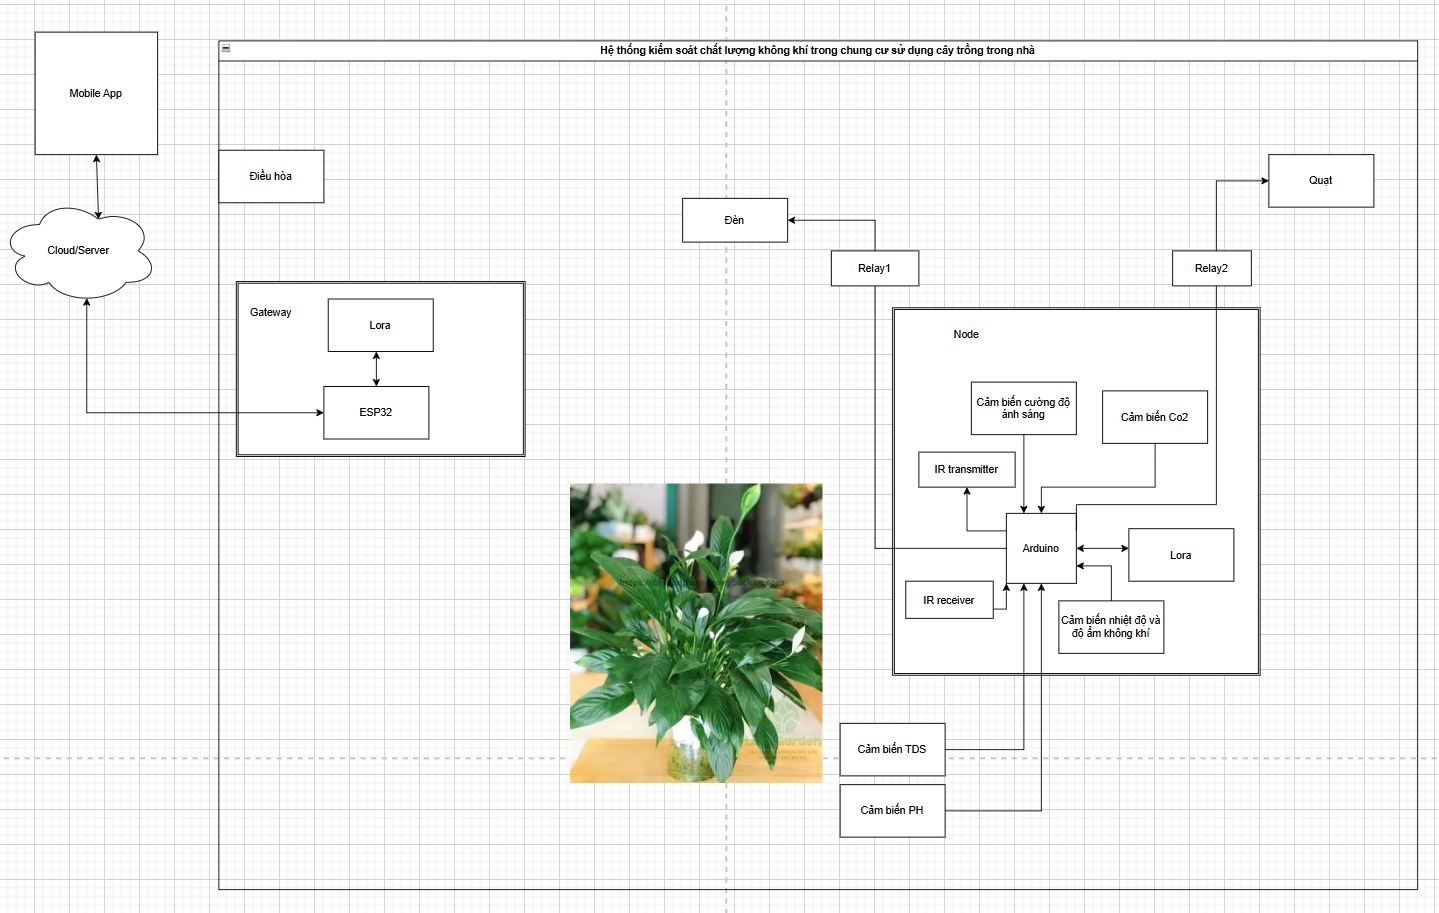
\includegraphics[width=\textwidth]{chapter5/image/kientruchethong.png}
    \caption{Kiến trúc tổng thể của hệ thống}
    \label{fig:system_architecture_overview}
\end{figure}

Hệ thống gồm bốn khối chính:
\begin{itemize}
    \item \textbf{Node cảm biến và điều khiển:} sử dụng Arduino Pro Mini để đọc TDS, pH, nhiệt độ, độ ẩm, CO2, ánh sáng và điều khiển relay, IR. Node đóng vai trò điểm đo tại khu vực cây trồng hoặc không gian sinh hoạt.
    \item \textbf{Kênh truyền LoRa:} truyền dữ liệu giữa node và gateway bằng hai module LoRa.
    \item \textbf{Gateway ESP32:} nhận dữ liệu từ node, gửi telemetry lên ThingsBoard và chuyển lệnh điều khiển từ ThingsBoard về node.
    \item \textbf{ThingsBoard và app Flutter:} lưu trữ, hiển thị dữ liệu, cảnh báo và cung cấp giao diện điều khiển cho người dùng.
\end{itemize}

Dữ liệu môi trường được thu thập định kỳ tại node. Sau khi đọc cảm biến, node chuẩn hóa dữ liệu, đóng gói và gửi qua LoRa. Gateway ESP32 giải mã gói tin, kiểm tra mã node, kiểm tra checksum nếu có và gửi dữ liệu lên ThingsBoard. Khi người dùng điều khiển quạt, đèn hoặc điều hòa trên app Flutter, lệnh được gửi đến ThingsBoard, gateway nhận lệnh và truyền xuống node qua LoRa. Nhờ đó, hệ thống hình thành vòng kín ở mức ứng dụng: đo lường, hiển thị, ra quyết định và phản hồi trạng thái.

\section{Luồng dữ liệu tổng quát}
Hệ thống được tổ chức theo hai luồng chính: luồng giám sát và luồng điều khiển. Luồng giám sát đi từ node lên app, còn luồng điều khiển đi từ app xuống node. Việc tách hai luồng này giúp thiết kế phần mềm rõ ràng và dễ kiểm thử.

Trong luồng giám sát, node đọc cảm biến theo chu kỳ. Các thông số gồm TDS, pH, ánh sáng, CO2, nhiệt độ và độ ẩm được đóng gói thành bản tin LoRa. Gateway nhận bản tin, chuyển đổi sang JSON và gửi lên ThingsBoard. App Flutter truy vấn dữ liệu từ ThingsBoard để hiển thị trên tab Sensor. Ảnh giao diện Sensor cho thấy các thông số được trình bày dưới dạng thẻ, mỗi thẻ có biểu tượng, tên đại lượng và giá trị hiện tại. Cách bố trí này giúp người dùng đọc nhanh trạng thái node trên màn hình điện thoại.

Trong luồng điều khiển, người dùng chuyển sang tab Actuator để điều khiển RL1, RL2 và điều hòa. Khi nhấn một thiết bị, app gửi lệnh đến ThingsBoard. Gateway nhận lệnh này và chuyển thành bản tin LoRa gửi tới node. Node thực thi lệnh, cập nhật trạng thái relay hoặc phát mã IR, sau đó gửi ACK về gateway. Gateway cập nhật lại trạng thái lên ThingsBoard để app hiển thị đúng.

\begin{figure}[h!]
    \centering
    \begin{tikzpicture}[node distance=1.3cm, every node/.style={font=\small}]
        \node[draw, rounded corners, minimum width=2.7cm, minimum height=0.9cm, fill=green!10] (node) {Node Arduino};
        \node[draw, rounded corners, right=of node, minimum width=2.7cm, minimum height=0.9cm, fill=green!10] (gateway) {ESP32 Gateway};
        \node[draw, rounded corners, right=of gateway, minimum width=2.7cm, minimum height=0.9cm, fill=green!10] (tb) {ThingsBoard};
        \node[draw, rounded corners, right=of tb, minimum width=2.7cm, minimum height=0.9cm, fill=green!10] (app) {Flutter App};
        \draw[->, thick] (node) -- node[above]{LoRa} (gateway);
        \draw[->, thick] (gateway) -- node[above]{MQTT/HTTP} (tb);
        \draw[->, thick] (tb) -- node[above]{API} (app);
        \draw[->, thick, bend right=35] (app) to node[below]{RPC} (tb);
        \draw[->, thick, bend right=35] (tb) to node[below]{lệnh} (gateway);
        \draw[->, thick, bend right=35] (gateway) to node[below]{LoRa} (node);
    \end{tikzpicture}
    \caption{Luồng dữ liệu hai chiều của hệ thống}
    \label{fig:data_control_flow}
\end{figure}

\section{Các chế độ vận hành}
Hệ thống có hai chế độ vận hành: tự động và thủ công. Trên giao diện app, công tắc \textit{Manual} thể hiện chế độ điều khiển bằng tay. Khi Manual được bật, người dùng chủ động bật/tắt relay và điều khiển điều hòa. Khi Manual tắt, hệ thống có thể áp dụng các luật điều khiển tự động dựa trên ngưỡng.

Chế độ thủ công phù hợp trong giai đoạn thử nghiệm vì người dùng có thể kiểm tra ngay phản hồi của từng actuator. Ví dụ, khi nhấn RL1, relay 1 phải đổi trạng thái; khi nhấn điều hòa, node phải phát mã IR. Chế độ tự động phù hợp khi hệ thống đã được hiệu chuẩn và người dùng đã xác định ngưỡng vận hành mong muốn. Các ngưỡng này có thể bao gồm bật quạt khi CO2 cao, bật đèn khi ánh sáng thấp, cảnh báo khi pH/TDS vượt vùng phù hợp hoặc gợi ý mở cửa khi phòng thiếu thông gió.

\begin{longtable}{|p{3cm}|p{4.5cm}|p{5.7cm}|}
\hline
\textbf{Chế độ} & \textbf{Nguồn quyết định} & \textbf{Ví dụ hành vi} \\
\hline
Manual & Người dùng trên app & Bật RL1, tắt RL2, tăng/giảm nhiệt độ điều hòa theo thao tác trực tiếp. \\
\hline
Auto & Luật điều khiển trong gateway hoặc ThingsBoard & Tự bật quạt khi CO2 cao, bật đèn khi ánh sáng thấp, cảnh báo khi pH/TDS bất thường. \\
\hline
\end{longtable}
